\documentclass[11pt]{article}
% Shared preamble of the RMC kernel write-ups (% Shared preamble of the RMC kernel write-ups (% Shared preamble of the RMC kernel write-ups (\input{preamble} after \documentclass).
\usepackage[margin=1in]{geometry}
\usepackage{amsmath,amssymb,bm}
\usepackage{graphicx}
\usepackage{booktabs}
\usepackage{hyperref}

\newcommand{\dd}{\,\mathrm{d}}
\newcommand{\Ein}{E}
\newcommand{\Eout}{E'}
\newcommand{\Ecm}{E_{c}}
\newcommand{\mucm}{\mu_{c}}
\newcommand{\mulab}{\mu_0}

% Common closing section: how the verification figures are produced
\newcommand{\verificationmethod}{%
Each figure is produced by \texttt{verification/verify\_laws.py}. For an incident
energy $\Ein$ along $+z$, $10^6$ collisions are sampled with MC/DC's own reaction
sampler (\texttt{sample\_elastic\_scattering}, \texttt{sample\_inelastic\_scattering}
or \texttt{sample\_fission}), and every emitted neutron is histogrammed in
$48 \times 24$ bins of $(\Eout, \mulab)$, with $\mulab$ the lab cosine to $+z$. The
inverted kernel used by RMC is integrated over the same bins (Gauss--Legendre panels;
two-body lines are split where $\mulab^*(\Eout)$ crosses a cosine edge), multiplied by
the number of collisions, and compared with a $\chi^2$ test over bins with at least 5
expected counts (the rest pooled into one bin). The tables list $\chi^2/\mathrm{dof}$,
its $p$-value, the emitted neutrons per collision (sampled vs.\ the integral of the
inverted kernel), and the largest relative change of a bin integral when the
quadrature panels are doubled. Left panels: outgoing-energy marginal; middle:
lab-cosine marginal; right: per-bin $z = (\text{sampled} - \text{inverted}) /
\sqrt{\text{inverted}}$.}
 after \documentclass).
\usepackage[margin=1in]{geometry}
\usepackage{amsmath,amssymb,bm}
\usepackage{graphicx}
\usepackage{booktabs}
\usepackage{hyperref}

\newcommand{\dd}{\,\mathrm{d}}
\newcommand{\Ein}{E}
\newcommand{\Eout}{E'}
\newcommand{\Ecm}{E_{c}}
\newcommand{\mucm}{\mu_{c}}
\newcommand{\mulab}{\mu_0}

% Common closing section: how the verification figures are produced
\newcommand{\verificationmethod}{%
Each figure is produced by \texttt{verification/verify\_laws.py}. For an incident
energy $\Ein$ along $+z$, $10^6$ collisions are sampled with MC/DC's own reaction
sampler (\texttt{sample\_elastic\_scattering}, \texttt{sample\_inelastic\_scattering}
or \texttt{sample\_fission}), and every emitted neutron is histogrammed in
$48 \times 24$ bins of $(\Eout, \mulab)$, with $\mulab$ the lab cosine to $+z$. The
inverted kernel used by RMC is integrated over the same bins (Gauss--Legendre panels;
two-body lines are split where $\mulab^*(\Eout)$ crosses a cosine edge), multiplied by
the number of collisions, and compared with a $\chi^2$ test over bins with at least 5
expected counts (the rest pooled into one bin). The tables list $\chi^2/\mathrm{dof}$,
its $p$-value, the emitted neutrons per collision (sampled vs.\ the integral of the
inverted kernel), and the largest relative change of a bin integral when the
quadrature panels are doubled. Left panels: outgoing-energy marginal; middle:
lab-cosine marginal; right: per-bin $z = (\text{sampled} - \text{inverted}) /
\sqrt{\text{inverted}}$.}
 after \documentclass).
\usepackage[margin=1in]{geometry}
\usepackage{amsmath,amssymb,bm}
\usepackage{graphicx}
\usepackage{booktabs}
\usepackage{hyperref}

\newcommand{\dd}{\,\mathrm{d}}
\newcommand{\Ein}{E}
\newcommand{\Eout}{E'}
\newcommand{\Ecm}{E_{c}}
\newcommand{\mucm}{\mu_{c}}
\newcommand{\mulab}{\mu_0}

% Common closing section: how the verification figures are produced
\newcommand{\verificationmethod}{%
Each figure is produced by \texttt{verification/verify\_laws.py}. For an incident
energy $\Ein$ along $+z$, $10^6$ collisions are sampled with MC/DC's own reaction
sampler (\texttt{sample\_elastic\_scattering}, \texttt{sample\_inelastic\_scattering}
or \texttt{sample\_fission}), and every emitted neutron is histogrammed in
$48 \times 24$ bins of $(\Eout, \mulab)$, with $\mulab$ the lab cosine to $+z$. The
inverted kernel used by RMC is integrated over the same bins (Gauss--Legendre panels;
two-body lines are split where $\mulab^*(\Eout)$ crosses a cosine edge), multiplied by
the number of collisions, and compared with a $\chi^2$ test over bins with at least 5
expected counts (the rest pooled into one bin). The tables list $\chi^2/\mathrm{dof}$,
its $p$-value, the emitted neutrons per collision (sampled vs.\ the integral of the
inverted kernel), and the largest relative change of a bin integral when the
quadrature panels are doubled. Left panels: outgoing-energy marginal; middle:
lab-cosine marginal; right: per-bin $z = (\text{sampled} - \text{inverted}) /
\sqrt{\text{inverted}}$.}


\title{Inverted kernel: Kalbach--Mann correlated energy--angle (ENDF Law 44)}
\date{}

\begin{document}
\maketitle

\noindent Code: \texttt{evaluate\_kalbach\_mann},
\texttt{\_correlated\_energy\_component}, \texttt{kalbach\_density} in
\texttt{mcdc/rmc/evaluate.py}.

\section{What MC/DC samples}

\texttt{sample\_kalbach\_mann}: an incident grid $E_l$ with outgoing tables
$\{E'_{l,k}, p_{l,k}, c_{l,k}, R_{l,k}, A_{l,k}\}$ (linear PDFs).
\begin{enumerate}
  \item Interpolation factor $f = (\Ein - E_i)/(E_{i+1} - E_i)$ and interpolated bounds
  $E'_{\min} = E'_{i,1} + f(E'_{i+1,1} - E'_{i,1})$,
  $E'_{\max} = E'_{i,K_i} + f(E'_{i+1,K_{i+1}} - E'_{i,K_i})$.
  \item Table $l = i$ with probability $1-f$, else $i+1$.
  \item $\hat E$ from table $l$ by exact inversion of its linear PDF on the interval
  $k$ with $c_{l,k} \le \xi < c_{l,k+1}$.
  \item $R$ and $A$ interpolated linearly in $\hat E$ on that interval (the
  \emph{unscaled} outgoing energy).
  \item $\mu$ from the Kalbach density
  $p(\mu \mid R, A) = \frac{A}{2\sinh A}\left[\cosh(A\mu) + R\sinh(A\mu)\right]$.
  \item Unit-base scaling $\Eout = E'_{\min} + (\hat E - E'_{l,1})
  (E'_{\max} - E'_{\min})/(E'_{l,K_l} - E'_{l,1})$.
\end{enumerate}
The pair $(\Eout, \mu)$ is in the reaction's frame (COM for the data used here).

\section{Inverted kernel}

For an outgoing energy $\Eout$, each table $l$ contributes through the unscaled energy
$\hat E_l(\Eout) = E'_{l,1} + (\Eout - E'_{\min})(E'_{l,K_l} - E'_{l,1})/(E'_{\max} -
E'_{\min})$ (zero if outside table $l$). With $k_l$ its interval,
$m_l = (\hat E_l - E'_{l,k})/(E'_{l,k+1} - E'_{l,k})$,
\begin{equation}
  f(\Eout, \mu \mid \Ein) = \sum_{l \in \{i, i+1\}} w_l\;
  p_{l}(\hat E_l)\,\frac{E'_{l,K_l} - E'_{l,1}}{E'_{\max} - E'_{\min}}\;
  \frac{A_l}{2\sinh A_l}\left[\cosh(A_l\mu) + R_l\sinh(A_l\mu)\right],
\end{equation}
$w_i = 1-f$, $w_{i+1} = f$, $p_l$ the linear PDF at $\hat E_l$,
$R_l = R_{l,k} + m_l(R_{l,k+1} - R_{l,k})$ and likewise $A_l$. The energy marginal is
exactly the scaled-table density; the angular factor integrates to 1 for each $l$. In
the COM frame $f_L = Y f(\Ecm, \mucm)\sqrt{\Eout/\Ecm}$. Kinks of the energy density
(table points mapped by the scaling) are quadrature breakpoints.

\section{Verification}
\verificationmethod

\begin{center}
\begin{tabular}{rrrrrrr}
\toprule
$E$ [eV] & samples & bins & $\chi^2/\mathrm{dof}$ & $p$ & yield (sampled / inverted) & quad. err. \\
\midrule
1.2e+07 & 1e+06 & 841 & 843.8/841 & 0.466 & 1.00000 / 1.00000 & 4.2e-04 \\
1.8e+07 & 1e+06 & 998 & 1021.1/998 & 0.299 & 1.00000 / 1.00000 & 4.9e-05 \\
\bottomrule
\end{tabular}

\end{center}

\begin{figure}[h]
  \centering
  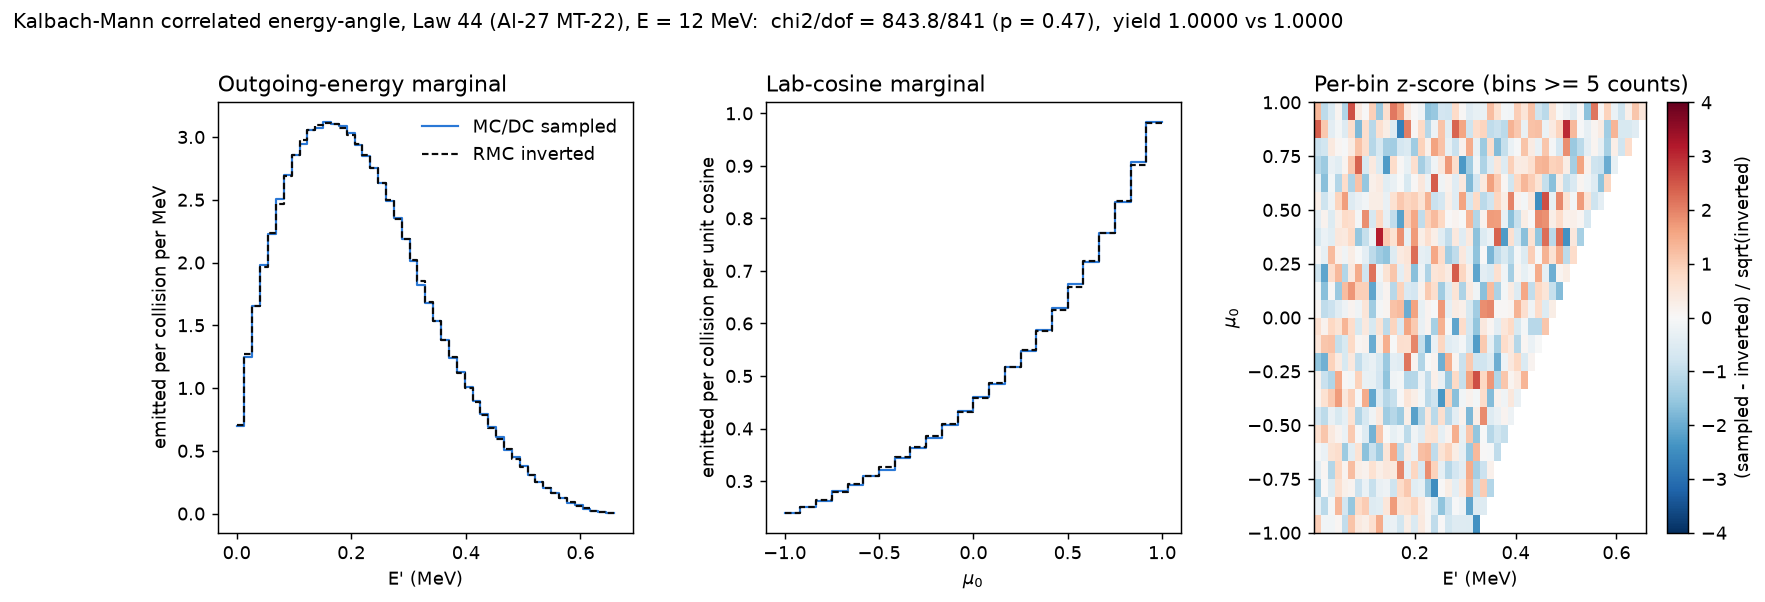
\includegraphics[width=\textwidth]{figures/kalbach_mann/kalbach_mann_E1p2e07.png}
  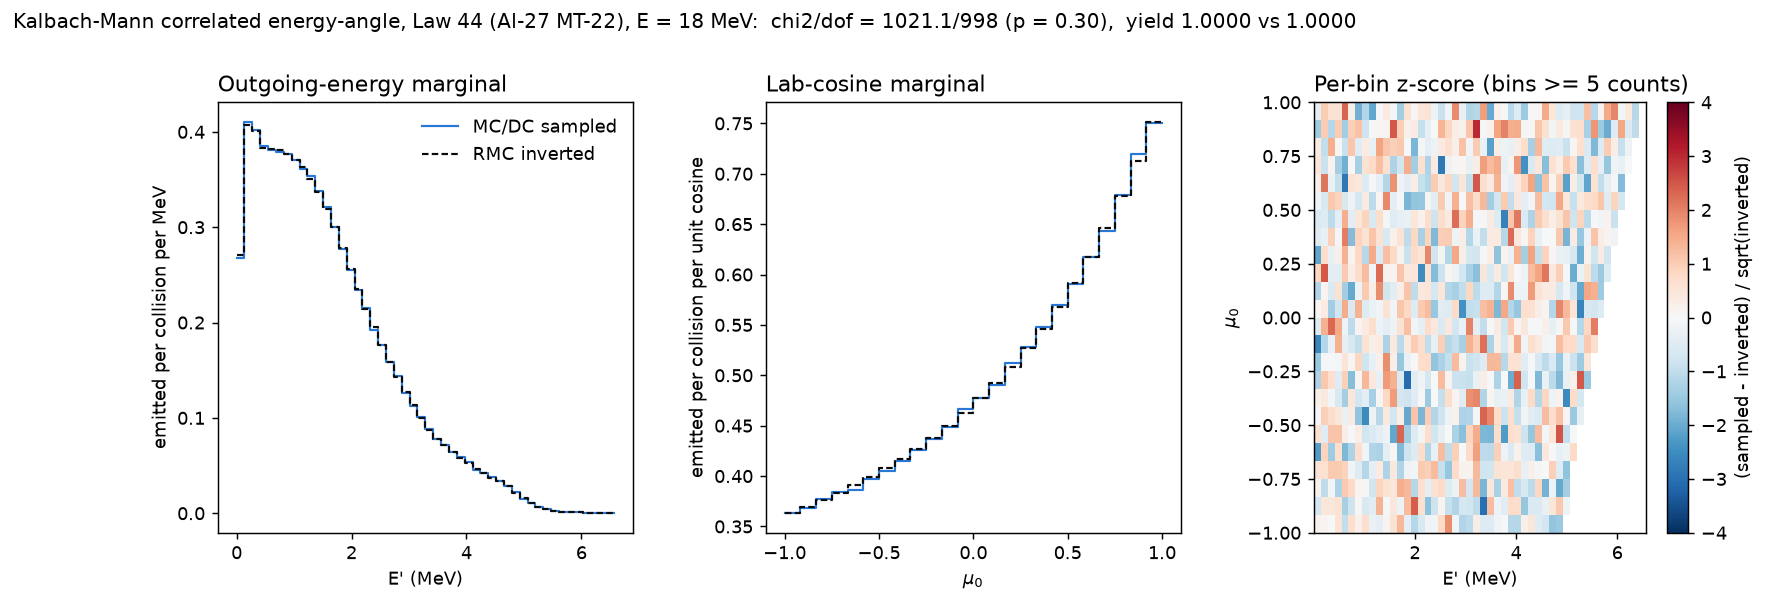
\includegraphics[width=\textwidth]{figures/kalbach_mann/kalbach_mann_E1p8e07.png}
  \caption{Al-27 MT-22 $(n,n\alpha)$, Kalbach--Mann in the COM frame, at 12 and
  18\,MeV.}
\end{figure}

\end{document}
